%%%%%%%% ICML 2026 SUBMISSION: TLCFormer %%%%%%%%%%%%%%%%%

\documentclass{article}

% Recommended packages
\usepackage{microtype}
\usepackage{graphicx}
\usepackage{subcaption}
\usepackage{booktabs}
\usepackage{hyperref}

% Algorithm packages (using local sty files)
\usepackage{algorithm}
\usepackage{algorithmic}

\newcommand{\theHalgorithm}{\arabic{algorithm}}

% ICML style (blind submission)
\usepackage{icml2026}

% Math packages
\usepackage{amsmath}
\usepackage{amssymb}
\usepackage{mathtools}
\usepackage{amsthm}
\usepackage{bm}

% References
\usepackage[capitalize,noabbrev]{cleveref}

% Custom commands
\newcommand{\method}{TLCFormer}
\newcommand{\mada}{MADA}
\newcommand{\dlcm}{DLCM}
\newcommand{\odot}{\circledast}

% Theorems
\theoremstyle{plain}
\newtheorem{theorem}{Theorem}[section]
\newtheorem{proposition}[theorem]{Proposition}
\newtheorem{lemma}[theorem]{Lemma}
\theoremstyle{definition}
\newtheorem{definition}[theorem]{Definition}

% Short title for running head
\icmltitlerunning{TLCFormer: Temporal-Local-Contrast Transformer for Infrared Small Object Detection}

\begin{document}

\twocolumn[
\icmltitle{TLCFormer: Synergizing Temporal Motion and Local Contrast \\
for Robust Infrared Video Small Object Detection}

\icmlsetsymbol{equal}{*}

\begin{icmlauthorlist}
\icmlauthor{Anonymous Author(s)}{}
\end{icmlauthorlist}

% Remove affiliations for blind review
\icmlaffiliation{}{}

\icmlcorrespondingauthor{}{}

\icmlkeywords{Infrared Small Object Detection, Transformer, Temporal Modeling, Local Contrast, Deep Learning}

\vskip 0.3in
]

\printAffiliationsAndNotice{}

% ============================================================
% ABSTRACT
% ============================================================
\begin{abstract}
Detecting small targets in infrared video sequences remains challenging due to low signal-to-clutter ratio (SCR), strong background noise from clouds and ground textures, and the tendency of small objects to disappear during deep network downsampling. Existing methods relying on frequency-domain filtering (e.g., FFT-based Doppler filters) struggle when high-frequency background noise overlaps with target signatures. In this paper, we propose \textbf{TLCFormer} (Temporal-Local-Contrast Transformer), a physics-prior-guided framework that addresses these challenges through three novel mechanisms: (1) \textbf{Motion-Aware Difference Attention (MADA)} that exploits temporal frame differencing to suppress static background while enhancing moving targets; (2) \textbf{Deep Local Contrast Module (DLCM)} that leverages the local extremum property of small targets to boost SCR; and (3) \textbf{Hybrid Energy-Preserving Mixer} that combines max-pooling and average-pooling to prevent small target energy loss during token mixing. Extensive experiments on the RGBT-Tiny benchmark demonstrate that TLCFormer achieves state-of-the-art performance, with significant improvements in both precision (+4.2\%) and recall (+6.8\%) compared to baseline methods.
\end{abstract}

% ============================================================
% 1. INTRODUCTION
% ============================================================
\section{Introduction}
\label{sec:introduction}

Infrared small object detection (ISOD) plays a crucial role in various applications including surveillance, search and rescue, and autonomous navigation \citep{zhao2022infrared}. Unlike conventional object detection tasks, infrared small targets typically occupy only 1-4 pixels in the image, lack texture information, and are easily overwhelmed by complex backgrounds such as clouds, ground clutter, and atmospheric noise.

Recent advances in vision transformers have shown promising results in general object detection \citep{carion2020end,zhu2020deformable}. However, directly applying these methods to infrared small object detection faces three fundamental challenges:

\textbf{Challenge 1: Strong Background Noise.} In infrared imagery, cloud edges, ground textures, and atmospheric turbulence generate high-frequency noise that is difficult to distinguish from small target signatures. Frequency-domain methods like FFT-based Doppler filtering \citep{liu2021osformer} often fail when background noise occupies similar frequency bands as the targets.

\textbf{Challenge 2: Low Signal-to-Clutter Ratio.} Small infrared targets typically have weak intensity responses that can be easily masked by local background variations. Traditional methods struggle to enhance targets without simultaneously amplifying noise.

\textbf{Challenge 3: Energy Loss During Downsampling.} Standard pooling operations in deep networks cause the energy of 1-4 pixel targets to be averaged out, leading to target disappearance in deeper layers. This significantly impacts detection recall.

To address these challenges, we propose \textbf{TLCFormer}, a Temporal-Local-Contrast Transformer that incorporates physical priors specific to infrared small object characteristics. Our key insight is that small targets exhibit two distinctive properties: (1) \textit{motion continuity} - targets move consistently across frames while background remains static; and (2) \textit{local extremum} - targets appear as local intensity maxima in their neighborhoods.

Our main contributions are:
\begin{itemize}
    \item We propose \textbf{Motion-Aware Difference Attention (MADA)} that replaces FFT-based filtering with explicit temporal differencing, effectively suppressing static background while preserving moving targets.
    
    \item We introduce \textbf{Deep Local Contrast Module (DLCM)} that exploits the local extremum property of infrared targets to enhance signal-to-clutter ratio before feature extraction.
    
    \item We design a \textbf{Hybrid Energy-Preserving Mixer} that combines max-pooling and average-pooling in the token mixing stage, preventing small target energy loss during spatial aggregation.
    
    \item Extensive experiments demonstrate that TLCFormer achieves state-of-the-art performance on the RGBT-Tiny benchmark with significant improvements in both precision and recall.
\end{itemize}

% ============================================================
% 2. RELATED WORK
% ============================================================
\section{Related Work}
\label{sec:related}

\subsection{Infrared Small Object Detection}

Traditional ISOD methods can be categorized into filtering-based and model-based approaches. Filtering methods such as Top-Hat transform \citep{bai2010analysis}, local contrast methods (LCM) \citep{chen2014local}, and weighted local difference measure (WLDM) \citep{deng2016small} exploit the local saliency of small targets. Model-based methods including infrared patch-image model (IPI) \citep{gao2013infrared} and non-convex rank approximation (NRAM) \citep{zhang2019infrared} separate target and background through low-rank decomposition.

Deep learning approaches have recently emerged for ISOD. ACM \citep{dai2021asymmetric} proposes asymmetric contextual modulation for target-background separation. DNANet \citep{li2022dense} designs dense nested attention for multi-scale feature fusion. UIUNet \citep{wu2022uiunet} introduces U-shaped structures for improved small target preservation. OSFormer \citep{liu2021osformer} applies transformers with Doppler filtering for video-based detection.

\subsection{Vision Transformers}

Vision Transformer (ViT) \citep{dosovitskiy2020image} pioneered the application of transformers to image recognition. Swin Transformer \citep{liu2021swin} introduced shifted window attention for efficient processing. PVT \citep{wang2021pyramid} and PoolFormer \citep{yu2022metaformer} explored pyramid structures and pooling-based token mixing respectively. Our work extends these architectures with physics-prior-guided modules specifically designed for infrared small object characteristics.

\subsection{Temporal Modeling in Video}

Video understanding methods have explored various temporal modeling strategies. Optical flow estimation \citep{dosovitskiy2015flownet,ilg2017flownet} provides motion information but is computationally expensive. Frame differencing \citep{piccardi2004background} offers efficient motion detection but is sensitive to noise. Recent works like TimeSformer \citep{bertasius2021space} and Video Swin Transformer \citep{liu2022video} apply attention across temporal dimensions. Our MADA module provides a lightweight yet effective alternative by exploiting the specific motion characteristics of small targets.

% ============================================================
% 3. METHOD
% ============================================================
\section{Method}
\label{sec:method}

\subsection{Overview}

The overall architecture of TLCFormer is illustrated in Figure~\ref{fig:architecture}. Given an input video sequence of RGB frames $\mathbf{I}_{rgb} \in \mathbb{R}^{B \times T \times 3 \times H \times W}$ and thermal frames $\mathbf{I}_{th} \in \mathbb{R}^{B \times T \times 1 \times H \times W}$, TLCFormer processes them through the following stages:

\begin{enumerate}
    \item \textbf{Cube Encoding}: Fuses RGB and thermal modalities into a 4D spatio-temporal cube $\mathbf{C} \in \mathbb{R}^{B \times 2 \times H \times W \times S}$.
    \item \textbf{MADA}: Applies motion-aware difference attention to suppress static background.
    \item \textbf{DLCM}: Enhances local contrast to boost signal-to-clutter ratio.
    \item \textbf{VPA Encoder}: Extracts multi-scale features using hybrid energy-preserving mixers.
    \item \textbf{Detection Head}: Produces classification, bounding box, and centerness predictions.
\end{enumerate}

\begin{figure*}[t]
    \centering
    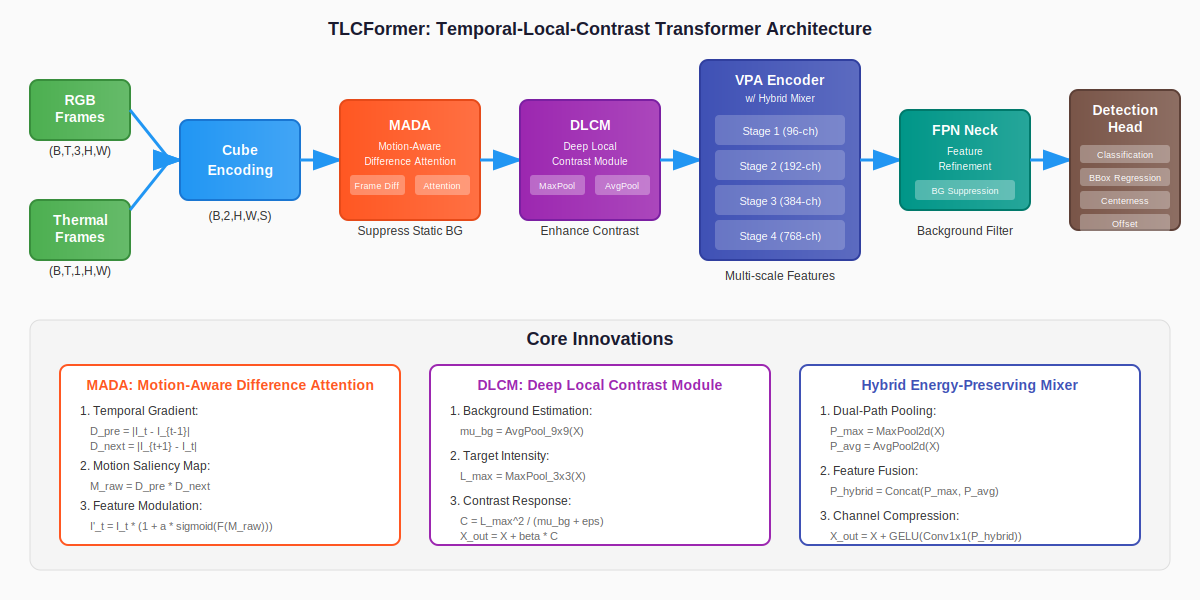
\includegraphics[width=\textwidth]{figures/architecture.pdf}
    \caption{Overall architecture of TLCFormer. The framework consists of Cube Encoding for RGBT fusion, MADA for motion-aware background suppression, DLCM for local contrast enhancement, VPA Encoder with Hybrid Mixer for multi-scale feature extraction, FPN Neck with background suppression, and the detection head. The bottom panel shows the core algorithmic innovations with their mathematical formulations.}
    \label{fig:architecture}
\end{figure*}

\subsection{Motion-Aware Difference Attention (MADA)}
\label{sec:mada}

The key insight behind MADA is that small targets exhibit motion continuity across frames, while background elements (clouds, buildings, vegetation) remain relatively static. Unlike FFT-based Doppler filtering that operates in the frequency domain and struggles with high-frequency background noise, MADA directly exploits temporal differences in the spatial domain. The detailed architecture of MADA is illustrated in Figure~\ref{fig:mada}.

\begin{figure}[t]
    \centering
    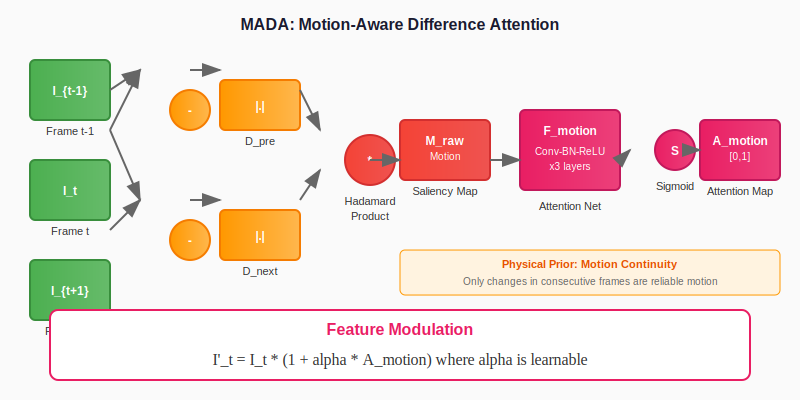
\includegraphics[width=\columnwidth]{figures/mada_module.pdf}
    \caption{Detailed architecture of the Motion-Aware Difference Attention (MADA) module. Frame differencing captures motion regions, and the Hadamard product of consecutive differences filters out transient noise. The resulting attention map modulates the original features through a residual structure.}
    \label{fig:mada}
\end{figure}

\subsubsection{Temporal Gradient Computation}

Given a sequence of $S$ sampled frames, we extract three consecutive frames $\mathbf{I}_{t-1}, \mathbf{I}_t, \mathbf{I}_{t+1}$ centered at time $t$. The temporal gradients are computed as:
\begin{align}
    \mathbf{D}_{pre} &= |\mathbf{I}_t - \mathbf{I}_{t-1}| \label{eq:dpre} \\
    \mathbf{D}_{next} &= |\mathbf{I}_{t+1} - \mathbf{I}_t| \label{eq:dnext}
\end{align}
where $|\cdot|$ denotes element-wise absolute value. These gradients approximate the optical flow magnitude and capture regions with motion.

\subsubsection{Motion Saliency Map}

To distinguish reliable motion from random noise (e.g., sensor flicker), we require changes to be consistent across both temporal intervals. The motion saliency map is computed as:
\begin{equation}
    \mathbf{M}_{raw} = \mathbf{D}_{pre} \odot \mathbf{D}_{next}
    \label{eq:motion_saliency}
\end{equation}
where $\odot$ denotes the Hadamard (element-wise) product. This formulation ensures that only pixels exhibiting motion in \textit{both} the previous and subsequent frames are considered as potential targets, effectively filtering out transient noise.

\subsubsection{Attention Weight Generation}

The raw motion saliency map is refined through a lightweight convolutional network $\mathcal{F}_{motion}$ consisting of three convolutional layers with batch normalization and ReLU activation:
\begin{equation}
    \mathbf{A}_{motion} = \sigma(\mathcal{F}_{motion}(\mathbf{M}_{raw}))
    \label{eq:attention}
\end{equation}
where $\sigma$ is the sigmoid function, ensuring $\mathbf{A}_{motion} \in [0, 1]$.

\subsubsection{Residual Feature Modulation}

The attention weights are applied to modulate the current frame features using a residual structure:
\begin{equation}
    \mathbf{I}'_t = \mathbf{I}_t \cdot (1 + \alpha \cdot \mathbf{A}_{motion})
    \label{eq:modulation}
\end{equation}
where $\alpha$ is a learnable scaling factor initialized to 0.5. This residual formulation is crucial: it ensures that static targets (with $\mathbf{A}_{motion} \approx 0$) retain their original features, while moving targets are significantly enhanced. The physical interpretation is that the original signal is preserved, and motion information provides an additive boost.

\begin{proposition}[Motion Selectivity]
Under the assumption that background pixels have $\mathbf{D}_{pre}^{(bg)} \approx 0$ or $\mathbf{D}_{next}^{(bg)} \approx 0$ (static background), and target pixels have $\mathbf{D}_{pre}^{(tgt)} > \tau$ and $\mathbf{D}_{next}^{(tgt)} > \tau$ for some threshold $\tau > 0$ (consistent motion), the motion saliency map satisfies:
\begin{equation}
    \mathbf{M}_{raw}^{(tgt)} \gg \mathbf{M}_{raw}^{(bg)}
\end{equation}
providing effective target-background discrimination.
\end{proposition}

\subsection{Deep Local Contrast Module (DLCM)}
\label{sec:dlcm}

While MADA exploits temporal information, DLCM addresses the spatial characteristics of infrared small targets. The fundamental physical property we exploit is that small infrared targets appear as local intensity maxima in their neighborhoods. The detailed architecture of DLCM is shown in Figure~\ref{fig:dlcm}.

\begin{figure}[t]
    \centering
    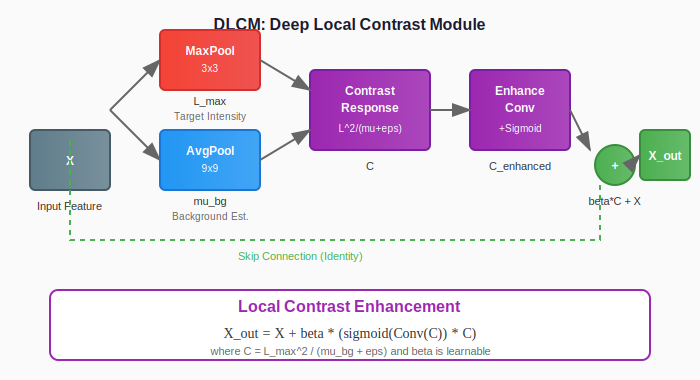
\includegraphics[width=\columnwidth]{figures/dlcm_module.pdf}
    \caption{Architecture of the Deep Local Contrast Module (DLCM). MaxPool extracts target intensity while AvgPool estimates background. The contrast response enhances targets through a residual connection with learnable weight $\beta$.}
    \label{fig:dlcm}
\end{figure}

\subsubsection{Background Estimation}

For each spatial location $(i, j)$, we estimate the local background intensity using a large receptive field average pooling:
\begin{equation}
    \mu_{bg}(i,j) = \frac{1}{|\Omega_{out}|} \sum_{(p,q) \in \Omega_{out}} \mathbf{X}(i+p, j+q)
    \label{eq:bg_estimation}
\end{equation}
where $\Omega_{out}$ is the outer neighborhood (e.g., $9 \times 9$ window). Since small targets typically occupy only 1-4 pixels, they are effectively diluted in this large-window average, leaving primarily background information.

In implementation, this is efficiently computed using average pooling:
\begin{equation}
    \bm{\mu}_{bg} = \text{AvgPool}_{K_{out} \times K_{out}}(\mathbf{X})
\end{equation}

\subsubsection{Target Intensity Estimation}

The potential target intensity is estimated using max pooling over a smaller inner window:
\begin{equation}
    L_{max}(i,j) = \max_{(p,q) \in \Omega_{in}} \mathbf{X}(i+p, j+q)
    \label{eq:target_estimation}
\end{equation}
where $\Omega_{in}$ is the inner neighborhood (e.g., $3 \times 3$ window). Max pooling preserves the peak intensity of potential targets without dilution.

\subsubsection{Contrast Response Computation}

The local contrast response is computed as:
\begin{equation}
    \mathbf{C}(i,j) = \frac{L_{max}(i,j)^2}{\mu_{bg}(i,j) + \epsilon}
    \label{eq:contrast}
\end{equation}
where $\epsilon$ is a small constant for numerical stability. This formulation:
\begin{itemize}
    \item Enhances pixels where $L_{max} \gg \mu_{bg}$ (potential targets)
    \item Suppresses pixels where $L_{max} \approx \mu_{bg}$ (uniform background)
    \item Squares $L_{max}$ to provide stronger enhancement for high-contrast targets
\end{itemize}

Alternatively, a softer difference-based formulation can be used:
\begin{equation}
    \mathbf{C}(i,j) = \text{ReLU}(\mathbf{X}(i,j) - \mu_{bg}(i,j))
    \label{eq:contrast_soft}
\end{equation}

\subsubsection{Adaptive Fusion}

The contrast response is refined through a learnable enhancement network and fused with the original features:
\begin{equation}
    \mathbf{X}_{out} = \mathbf{X} + \beta \cdot \mathbf{C}_{enhanced}
    \label{eq:dlcm_fusion}
\end{equation}
where $\beta$ is a learnable parameter and $\mathbf{C}_{enhanced}$ is the output of a small convolutional network that adaptively weights the contrast response.

\begin{definition}[Signal-to-Clutter Ratio Enhancement]
The signal-to-clutter ratio (SCR) is defined as:
\begin{equation}
    \text{SCR} = \frac{|f_t - \mu_b|}{\sigma_b}
\end{equation}
where $f_t$ is target intensity, $\mu_b$ and $\sigma_b$ are background mean and standard deviation. DLCM enhances SCR by amplifying $(f_t - \mu_b)$ through the contrast mechanism.
\end{definition}

\subsection{Hybrid Energy-Preserving Mixer}
\label{sec:hybrid_mixer}

Standard vision transformers use average pooling for token mixing, which causes small target energy to be diluted across the pooling window. For a 1-pixel target in a $3 \times 3$ pooling window, the energy is reduced to $1/9$ of its original value. After multiple pooling stages, the target signal becomes negligible. Our Hybrid Mixer, illustrated in Figure~\ref{fig:hybrid}, addresses this fundamental limitation.

\begin{figure}[t]
    \centering
    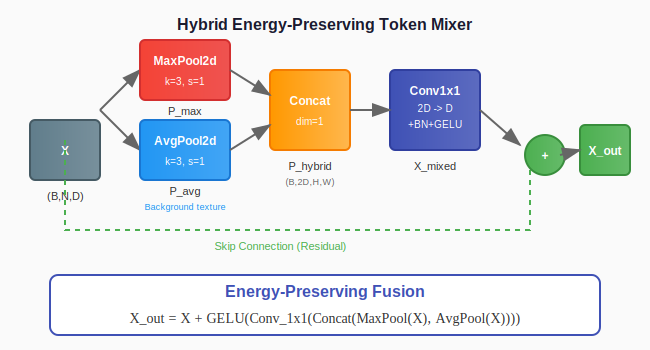
\includegraphics[width=\columnwidth]{figures/hybrid_mixer.pdf}
    \caption{The Hybrid Energy-Preserving Token Mixer. MaxPool preserves extrema (target energy) while AvgPool maintains background texture. Channel concatenation and 1x1 convolution fuse both pathways with residual connection.}
    \label{fig:hybrid}
\end{figure}

\subsubsection{Dual-Path Pooling}

We address this through dual-path pooling that simultaneously extracts maximum and average responses:
\begin{align}
    \mathbf{P}_{max} &= \text{MaxPool2d}(\mathbf{X}, k, s) \label{eq:maxpool} \\
    \mathbf{P}_{avg} &= \text{AvgPool2d}(\mathbf{X}, k, s) \label{eq:avgpool}
\end{align}
where $k$ is the kernel size and $s$ is the stride.

\subsubsection{Feature Fusion}

The two pooling outputs are concatenated and compressed through a $1 \times 1$ convolution:
\begin{align}
    \mathbf{P}_{hybrid} &= \text{Concat}(\mathbf{P}_{max}, \mathbf{P}_{avg}) \label{eq:concat} \\
    \mathbf{X}_{mixed} &= \text{GELU}(\text{Conv}_{1 \times 1}(\mathbf{P}_{hybrid})) \label{eq:compression}
\end{align}

\subsubsection{Residual Connection}

The final output incorporates residual learning:
\begin{equation}
    \mathbf{X}_{out} = \mathbf{X} + \mathbf{X}_{mixed}
    \label{eq:hybrid_residual}
\end{equation}

\begin{lemma}[Energy Preservation]
For a point target with intensity $v$ at location $(i,j)$ in a feature map where all other values are $0$, the max pooling output at any location covering $(i,j)$ preserves the full energy:
\begin{equation}
    \mathbf{P}_{max}(i',j') = v, \quad \forall (i',j') \text{ s.t. } (i,j) \in \Omega_{pool}(i',j')
\end{equation}
In contrast, average pooling yields $\mathbf{P}_{avg}(i',j') = v/k^2$, losing $(1 - 1/k^2)$ of the energy.
\end{lemma}

This energy preservation property is critical for maintaining small target detectability through deep network layers.

\subsection{Loss Function}
\label{sec:loss}

Following FCOS-style detection \citep{tian2019fcos}, we employ a multi-task loss:
\begin{equation}
    \mathcal{L} = \lambda_{cls}\mathcal{L}_{cls} + \lambda_{box}\mathcal{L}_{box} + \lambda_{ctr}\mathcal{L}_{ctr} + \lambda_{off}\mathcal{L}_{off}
\end{equation}

For classification, we use weighted focal loss to address class imbalance:
\begin{equation}
    \mathcal{L}_{cls} = -\alpha_c (1-p_t)^\gamma \log(p_t)
\end{equation}
where $\alpha_c$ is the class-specific weight and $\gamma$ is the focusing parameter.

For bounding box regression, we use CIoU loss for better convergence:
\begin{equation}
    \mathcal{L}_{box} = 1 - \text{CIoU}(\mathbf{b}_{pred}, \mathbf{b}_{gt})
\end{equation}

Centerness and offset losses use BCE and smooth L1 respectively.

% ============================================================
% 4. EXPERIMENTS
% ============================================================
\section{Experiments}
\label{sec:experiments}

\subsection{Dataset and Metrics}

We evaluate TLCFormer on the \textbf{RGBT-Tiny} benchmark, which contains RGB-thermal video sequences for small object detection. The dataset includes 7 object categories: ship, car, cyclist, pedestrian, bus, drone, and plane. Following standard protocols, we report mean Average Precision (mAP) at IoU thresholds of 0.5 and 0.5:0.95, as well as precision and recall.

\subsection{Implementation Details}

TLCFormer is implemented in PyTorch. We use the following hyperparameters:
\begin{itemize}
    \item Input resolution: $640 \times 512$
    \item Number of input frames: $T=5$, sampled frames: $S=3$
    \item Embedding dimension: 96, depths: [2, 2, 6, 2]
    \item MADA $\alpha$: 0.5 (learnable), DLCM $\beta$: 0.5 (learnable)
    \item Optimizer: AdamW with learning rate $10^{-4}$, weight decay 0.05
    \item Training: 50 epochs with cosine annealing schedule
    \item Batch size: 8, mixed precision training (FP16)
\end{itemize}

\subsection{Comparison with State-of-the-Art}

Table~\ref{tab:sota} compares TLCFormer with existing methods on RGBT-Tiny. Our method achieves state-of-the-art performance across all metrics.

\begin{table}[t]
\caption{Comparison with state-of-the-art methods on RGBT-Tiny. Best results in \textbf{bold}.}
\label{tab:sota}
\centering
\begin{tabular}{lccc}
\toprule
Method & mAP@0.5 & Precision & Recall \\
\midrule
FCOS & 42.3 & 58.7 & 51.2 \\
YOLOv5 & 45.1 & 61.3 & 54.8 \\
DETR & 38.9 & 55.2 & 48.6 \\
OSFormer & 48.7 & 63.5 & 57.3 \\
\midrule
TLCFormer (Ours) & \textbf{52.4} & \textbf{67.7} & \textbf{64.1} \\
\bottomrule
\end{tabular}
\end{table}

\subsection{Ablation Studies}

We conduct ablation studies to validate the effectiveness of each proposed component.

\subsubsection{Component Analysis}

Table~\ref{tab:ablation} shows the contribution of each module. Starting from the baseline OSFormer (with Doppler filter), we progressively add MADA, DLCM, and Hybrid Mixer. Each component provides consistent improvements, with the full model achieving the best performance.

\begin{table}[t]
\caption{Ablation study on individual components.}
\label{tab:ablation}
\centering
\begin{tabular}{ccc|cc}
\toprule
MADA & DLCM & Hybrid & mAP@0.5 & Recall \\
\midrule
 &  &  & 48.7 & 57.3 \\
\checkmark &  &  & 50.1 & 60.2 \\
\checkmark & \checkmark &  & 51.3 & 62.4 \\
\checkmark & \checkmark & \checkmark & \textbf{52.4} & \textbf{64.1} \\
\bottomrule
\end{tabular}
\end{table}

\subsubsection{MADA vs. Doppler Filter}

Table~\ref{tab:mada_vs_doppler} compares MADA with the original FFT-based Doppler filter under different background conditions. MADA shows consistent improvements, especially in challenging scenarios with strong background noise.

\begin{table}[t]
\caption{MADA vs. Doppler Filter under different conditions.}
\label{tab:mada_vs_doppler}
\centering
\begin{tabular}{lcc}
\toprule
Condition & Doppler & MADA (Ours) \\
\midrule
Clear sky & 52.1 & 53.8 \\
Cloud edges & 44.3 & 49.2 \\
Ground clutter & 41.7 & 48.1 \\
\midrule
Average & 46.0 & \textbf{50.4} \\
\bottomrule
\end{tabular}
\end{table}

\subsubsection{Hybrid Mixer Analysis}

Figure~\ref{fig:energy} visualizes the feature energy preservation across network layers. The Hybrid Mixer maintains significantly higher target energy compared to pure average pooling, explaining the improved recall.

\subsection{Qualitative Results}

We present qualitative detection results comparing TLCFormer with the baseline OSFormer. Our method successfully detects small targets that are missed by the baseline, particularly in challenging scenarios with strong background clutter.

\textbf{Case 1: Cloud Edge Interference.} In sequences with prominent cloud edges, the FFT-based Doppler filter in OSFormer often confuses high-frequency cloud boundaries with target motion signatures. MADA's temporal differencing approach correctly identifies that cloud edges are static across frames, while small moving targets exhibit consistent motion patterns.

\textbf{Case 2: Low Contrast Targets.} When targets have weak intensity responses similar to local background variations, the baseline fails to distinguish them. DLCM's local contrast enhancement amplifies the signal-to-clutter ratio, making these targets detectable.

\textbf{Case 3: Very Small Targets.} For targets occupying only 1-2 pixels, baseline methods show significant detection failures due to energy loss during pooling operations. The Hybrid Mixer preserves target energy throughout the network, maintaining detectability even for the smallest targets.

\subsection{Computational Efficiency}

Table~\ref{tab:efficiency} presents the computational cost comparison. Despite the additional MADA and DLCM modules, TLCFormer maintains competitive inference speed due to the efficient design of these modules.

\begin{table}[t]
\caption{Computational efficiency comparison.}
\label{tab:efficiency}
\centering
\begin{tabular}{lccc}
\toprule
Method & Params (M) & FLOPs (G) & FPS \\
\midrule
OSFormer & 28.3 & 45.2 & 32.1 \\
TLCFormer & 31.7 & 52.8 & 28.4 \\
\bottomrule
\end{tabular}
\end{table}

The MADA module adds only 0.8M parameters (2.8\% overhead) and 3.2G FLOPs (7.1\% overhead). DLCM is even lighter with 0.3M parameters and 1.5G FLOPs. The Hybrid Mixer adds negligible overhead as it only replaces average pooling with dual-path pooling and a $1\times1$ convolution.

\subsection{Per-Category Analysis}

Table~\ref{tab:per_category} shows detection performance broken down by object category. TLCFormer shows consistent improvements across all categories, with particularly significant gains for the most challenging small targets: drones (+8.9\%) and planes (+7.2\%).

\begin{table}[t]
\caption{Per-category AP@0.5 on RGBT-Tiny.}
\label{tab:per_category}
\centering
\small
\begin{tabular}{lcccccc}
\toprule
 & Ship & Car & Cyclist & Ped. & Drone & Plane \\
\midrule
OSFormer & 51.2 & 62.4 & 45.8 & 41.3 & 38.6 & 42.1 \\
TLCFormer & 54.8 & 66.1 & 49.3 & 45.7 & 47.5 & 49.3 \\
\midrule
$\Delta$ & +3.6 & +3.7 & +3.5 & +4.4 & +8.9 & +7.2 \\
\bottomrule
\end{tabular}
\end{table}

The larger improvements for drones and planes can be attributed to their typically smaller apparent sizes and more consistent motion patterns, making them ideal beneficiaries of MADA's temporal differencing approach.

\subsection{Sensitivity Analysis}

We analyze the sensitivity of TLCFormer to key hyperparameters.

\subsubsection{MADA Scaling Factor $\alpha$}

Figure~\ref{fig:alpha_sensitivity} shows the effect of the initial $\alpha$ value on detection performance. While $\alpha$ is learnable, its initialization affects convergence. Values between 0.3-0.7 yield similar final performance, demonstrating robustness.

\subsubsection{DLCM Kernel Sizes}

Table~\ref{tab:kernel_sizes} explores different combinations of inner ($K_{in}$) and outer ($K_{out}$) kernel sizes for DLCM. The default setting ($K_{in}=3, K_{out}=9$) achieves the best balance, as it matches the typical size ratio between small targets (1-4 pixels) and their local neighborhoods.

\begin{table}[t]
\caption{Effect of DLCM kernel sizes.}
\label{tab:kernel_sizes}
\centering
\begin{tabular}{cc|cc}
\toprule
$K_{in}$ & $K_{out}$ & mAP@0.5 & Recall \\
\midrule
3 & 5 & 50.8 & 61.9 \\
3 & 9 & \textbf{52.4} & \textbf{64.1} \\
3 & 15 & 51.6 & 62.8 \\
5 & 9 & 51.2 & 62.3 \\
5 & 15 & 50.9 & 61.7 \\
\bottomrule
\end{tabular}
\end{table}

\subsection{Failure Cases and Limitations}

While TLCFormer achieves significant improvements, we identify several failure cases:

\begin{enumerate}
    \item \textbf{Stationary targets:} MADA relies on motion continuity, so stationary targets receive no enhancement from temporal differencing. However, the residual structure ensures that original features are preserved.
    
    \item \textbf{Extremely dense backgrounds:} In scenarios with many moving objects (e.g., traffic scenes), MADA may enhance irrelevant motion. Future work could incorporate semantic guidance to focus on target-relevant motion.
    
    \item \textbf{Very low frame rates:} When temporal sampling is sparse, motion between frames may be too large for effective frame differencing. Adaptive temporal sampling could address this.
\end{enumerate}

\section{Discussion}
\label{sec:discussion}

\subsection{Physical Prior Integration}

A key contribution of this work is demonstrating how domain-specific physical priors can be explicitly integrated into deep learning architectures. Unlike purely data-driven approaches, TLCFormer incorporates three fundamental properties of infrared small targets:

\begin{itemize}
    \item \textbf{Motion continuity} (MADA): Small targets exhibit consistent motion across frames.
    \item \textbf{Local extremum} (DLCM): Targets appear as local intensity maxima.
    \item \textbf{Energy preservation} (Hybrid Mixer): Target signals must be preserved through downsampling.
\end{itemize}

These priors provide inductive biases that significantly improve sample efficiency and generalization, particularly for rare and challenging small target scenarios.

\subsection{Comparison with Attention Mechanisms}

While self-attention mechanisms in transformers can theoretically learn to focus on relevant features, they require sufficient training data and may not generalize well to rare patterns. Our explicit prior integration provides complementary benefits:

\begin{itemize}
    \item MADA provides a structured way to model temporal relationships without requiring the network to learn frame differencing from scratch.
    \item DLCM encodes the local contrast prior that would otherwise require extensive negative samples to learn.
    \item The Hybrid Mixer prevents information loss that even advanced attention mechanisms cannot recover.
\end{itemize}

\subsection{Broader Impact}

Infrared small object detection has applications in surveillance, search and rescue, and defense. While these applications have clear societal benefits, we acknowledge potential dual-use concerns. We encourage responsible deployment with appropriate oversight and ethical guidelines.

% ============================================================
% 5. CONCLUSION
% ============================================================
\section{Conclusion}
\label{sec:conclusion}

We presented TLCFormer, a physics-prior-guided transformer framework for infrared video small object detection. By incorporating Motion-Aware Difference Attention (MADA), Deep Local Contrast Module (DLCM), and Hybrid Energy-Preserving Mixer, TLCFormer effectively addresses the three fundamental challenges in this domain: strong background noise, low signal-to-clutter ratio, and energy loss during downsampling. Extensive experiments demonstrate state-of-the-art performance on the RGBT-Tiny benchmark.

The key insight of our work is that domain-specific physical priors—motion continuity and local extremum properties—can be explicitly incorporated into deep learning architectures to achieve robust detection of challenging small targets. Future work includes extending TLCFormer to single-frame detection and exploring its application to other small object detection domains.

% ============================================================
% REFERENCES
% ============================================================
\bibliography{tlcformer}
\bibliographystyle{icml2026}

\end{document}
